\documentclass{article}
\usepackage[margin=1.5in, includeheadfoot]{geometry}
\usepackage{fancyhdr}
\usepackage[fleqn]{amsmath}
\usepackage{amssymb, amsthm}
\usepackage{microtype}
\usepackage[shortlabels]{enumitem}
\usepackage{listings}
\usepackage{xcolor}
\usepackage{booktabs}
\usepackage[]{float}
\usepackage{graphicx}
\usepackage{subfig}
\usepackage{fullpage}
\graphicspath{ {./images/} }

\definecolor{codegreen}{rgb}{0,0.6,0}
\definecolor{codegray}{rgb}{0.5,0.5,0.5}
\definecolor{codepurple}{rgb}{0.58,0,0.82}
\definecolor{backcolour}{rgb}{0.95,0.95,0.92}
\lstdefinestyle{mystyle}{
    % backgroundcolor=\color{backcolour},   
    commentstyle=\color{codegreen},
    keywordstyle=\color{magenta},
    % numberstyle=\tiny\color{codegray},
    stringstyle=\color{codepurple},
    basicstyle=\ttfamily\footnotesize,
    breakatwhitespace=false,         
    breaklines=true,                 
    captionpos=b,                    
    keepspaces=true,                 
    numbers=left,                    
    numbersep=5pt,                  
    showspaces=false,                
    showstringspaces=false,
    showtabs=false,                  
    tabsize=2
}
\lstset{style=mystyle}

\linespread{1.2}

\author{Gus Beringer}
\title{Capstone Project}

\date{\today}
\newtheorem{theorem}{Theorem}
\def\D{\mathbb{D}}
\def\I{\mathbb{I}}
\def\N{\mathbb{N}}
\def\R{\mathbb{R}}
\def\T{\mathbb{T}}
\def\U{\mathbb{U}}
\def\Z{\mathbb{Z}}
\def\vep{{\varepsilon}}



\begin{document}
\maketitle
% \tableofcontents

\section{Introduction}

Every Wikipedia article contains links to other articles. If the article references a concept that is also another Wikipedia article, the text can link to that article.
The Wikipedia hyperlink graph is the graph with every article as a vertex. The edges between the vertices are the links between the articles.

It is observable that the Wikipedia hyperlink graph is a small world network.
A small-world network is a graph where each vertex is connected to few vertices, but can reach all other vertices within a few steps.

An undirected graph is connected when there is a path between any two vertices in the graph.
If there is a path between any two vertices in a directed graph, it is a strongly connected.
If a directed graph has an undirected graph that is connected, it is weakly connected.


\section{Sparse Adjacency Matrices}

The size of the wikipedia hyperlink graph presents challenges for computing any graph properties.
% The wikipedia hyperlink graph has over 6 million vertices.
It is not trivial to construct the adjacency matrix of the graph without overflowing computer memory.
The most popular graph package in python, Networkx, runs out of RAM within a minute.
% The hardest part of constructing the hyperlink graph in memory is the enormous size of the graph.
% When constructing the graph using the most common graph package in Python, network, the program quickly runs out of memory.
The Wikipedia hyperlink graph has 6,102,910 vertices.
Therefore, a dense representation of the adjacency matrix would need over $3.7 * 10^{13}$ units of storage for each cell in the matrix.
This is clearly not scalable.
Since most pages only have 100 links, there is clearly a more efficient way to store the matrix.

We employ sparse matrices to efficiently store the adjacency matrix of the graph in memory.
Instead of storing the whole adjacency matrix, a sparse matrix stores only the location of non-zero elements.
We use the compressed sparse row format to store the matrix.

The Python package scipy provides an implementation of the csr matrix format holds three arrays that make up the graph. The \textbf{data} array contains the values for the non-zero elements in the matrix. The \textbf{indices} array is the same length of the data array and contains the index of the corresponding column for each non-zero element. The \textbf{indptr} array contains the number of elements for each row in the matrix. With this information, the entire matrix can be accurately represented efficiently in memory. With the sparse format, the entire adjacency matrix can be represented with less than 4GB of memory.




\section{Degree Distribution}

We describe the distribution for the indegree and outdegree of the strongly connected network.


The indegree distribution has a smooth exponential descent. Most of the network has a small indegree. We find that 93.84\% of the network has a indegree smaller than 300. However, there are still plenty of nodes with large indegree. We find that 1.468 of vertices in the network have indegree larger than 10,000.

The outdegree distribution grows before declining. It has a much smaller maximum of 11,897 vertices. This is because the outdegree is limited by the size of the article, but the indegree is only limited by the relevance of the article and the size of the graph.


\begin{figure}[H]
    \centering
    \caption[]{Degree Statistics}
    \begin{tabular}{lrrrrr}
        \toprule
        & Q1 & Median & Mean & Q3 & Maximum\\
        \midrule
        Outdegree & 4 & 19 & 91.46176 & 81 & 1,305,902\\
        Indegree & 17 & 39 & 91.46176 & 107 & 11,897\\
        \bottomrule
    \end{tabular}
\end{figure}

\begin{figure}[H]
    \centering
    \parbox{6cm}{
    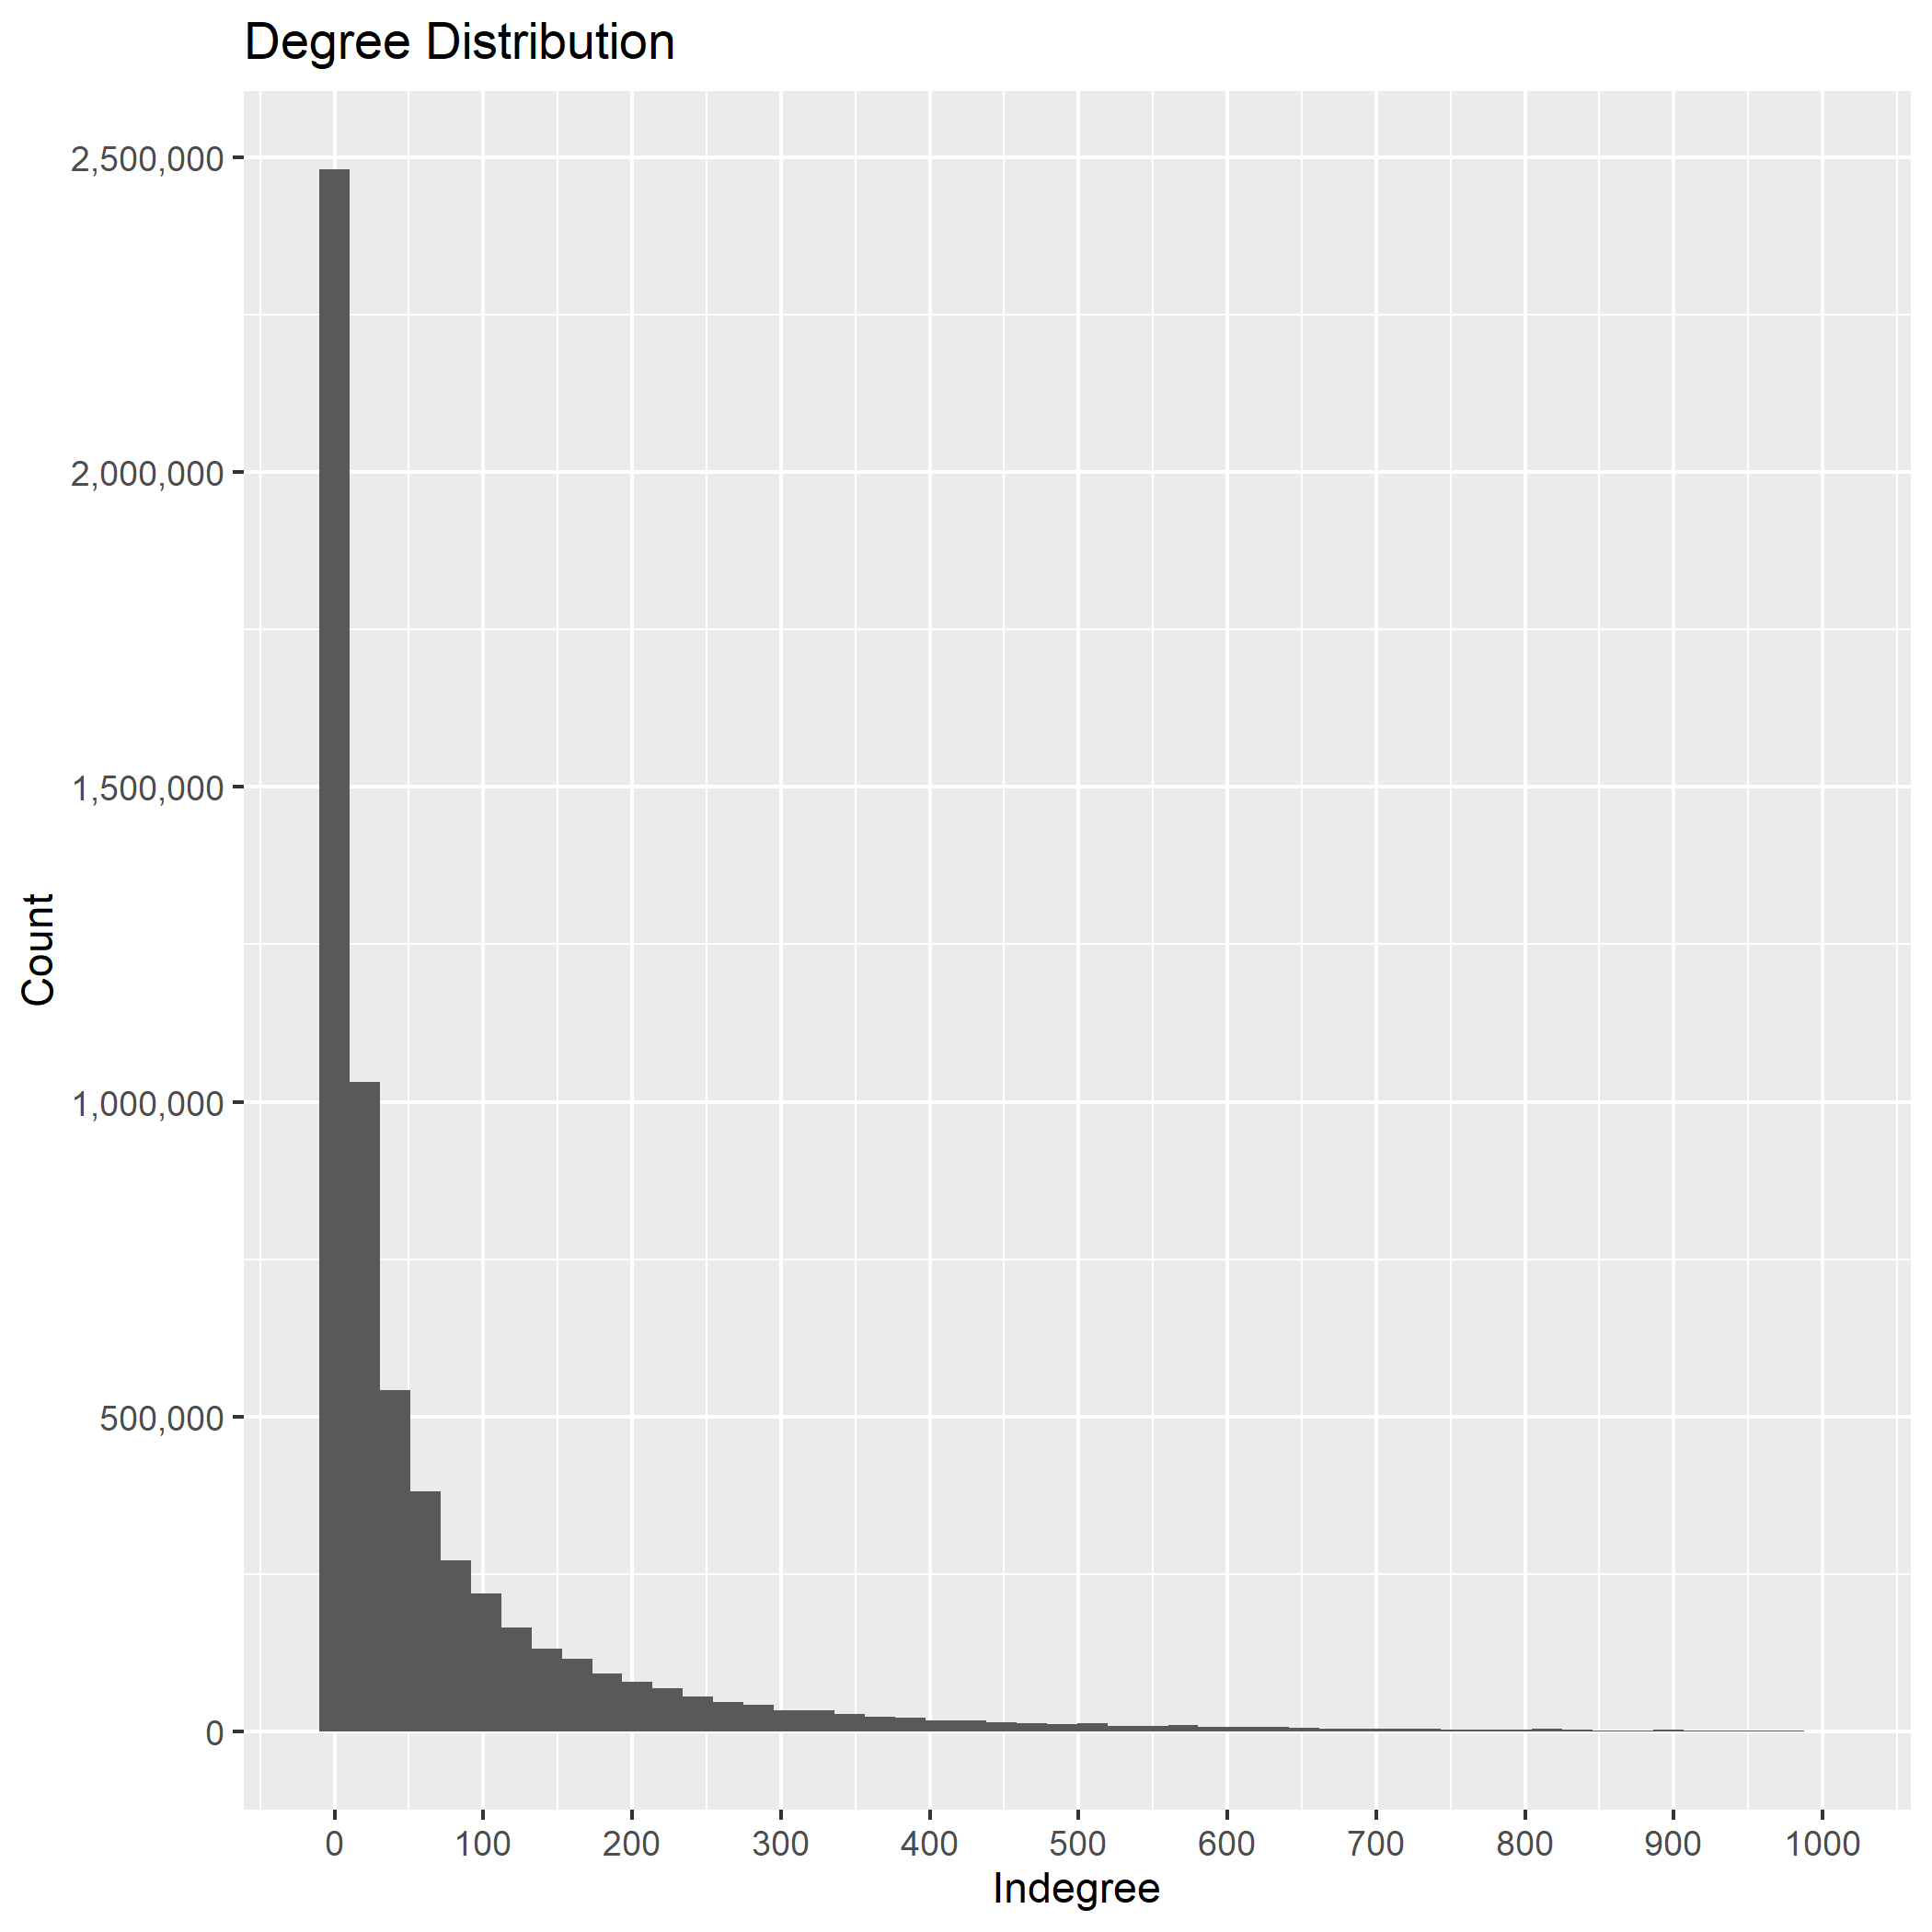
\includegraphics[width=6cm]{in_degree_dist}
    \caption{Indegree Distribution}
    \label{fig:2figsA}}
    \qquad
    \begin{minipage}{6cm}
    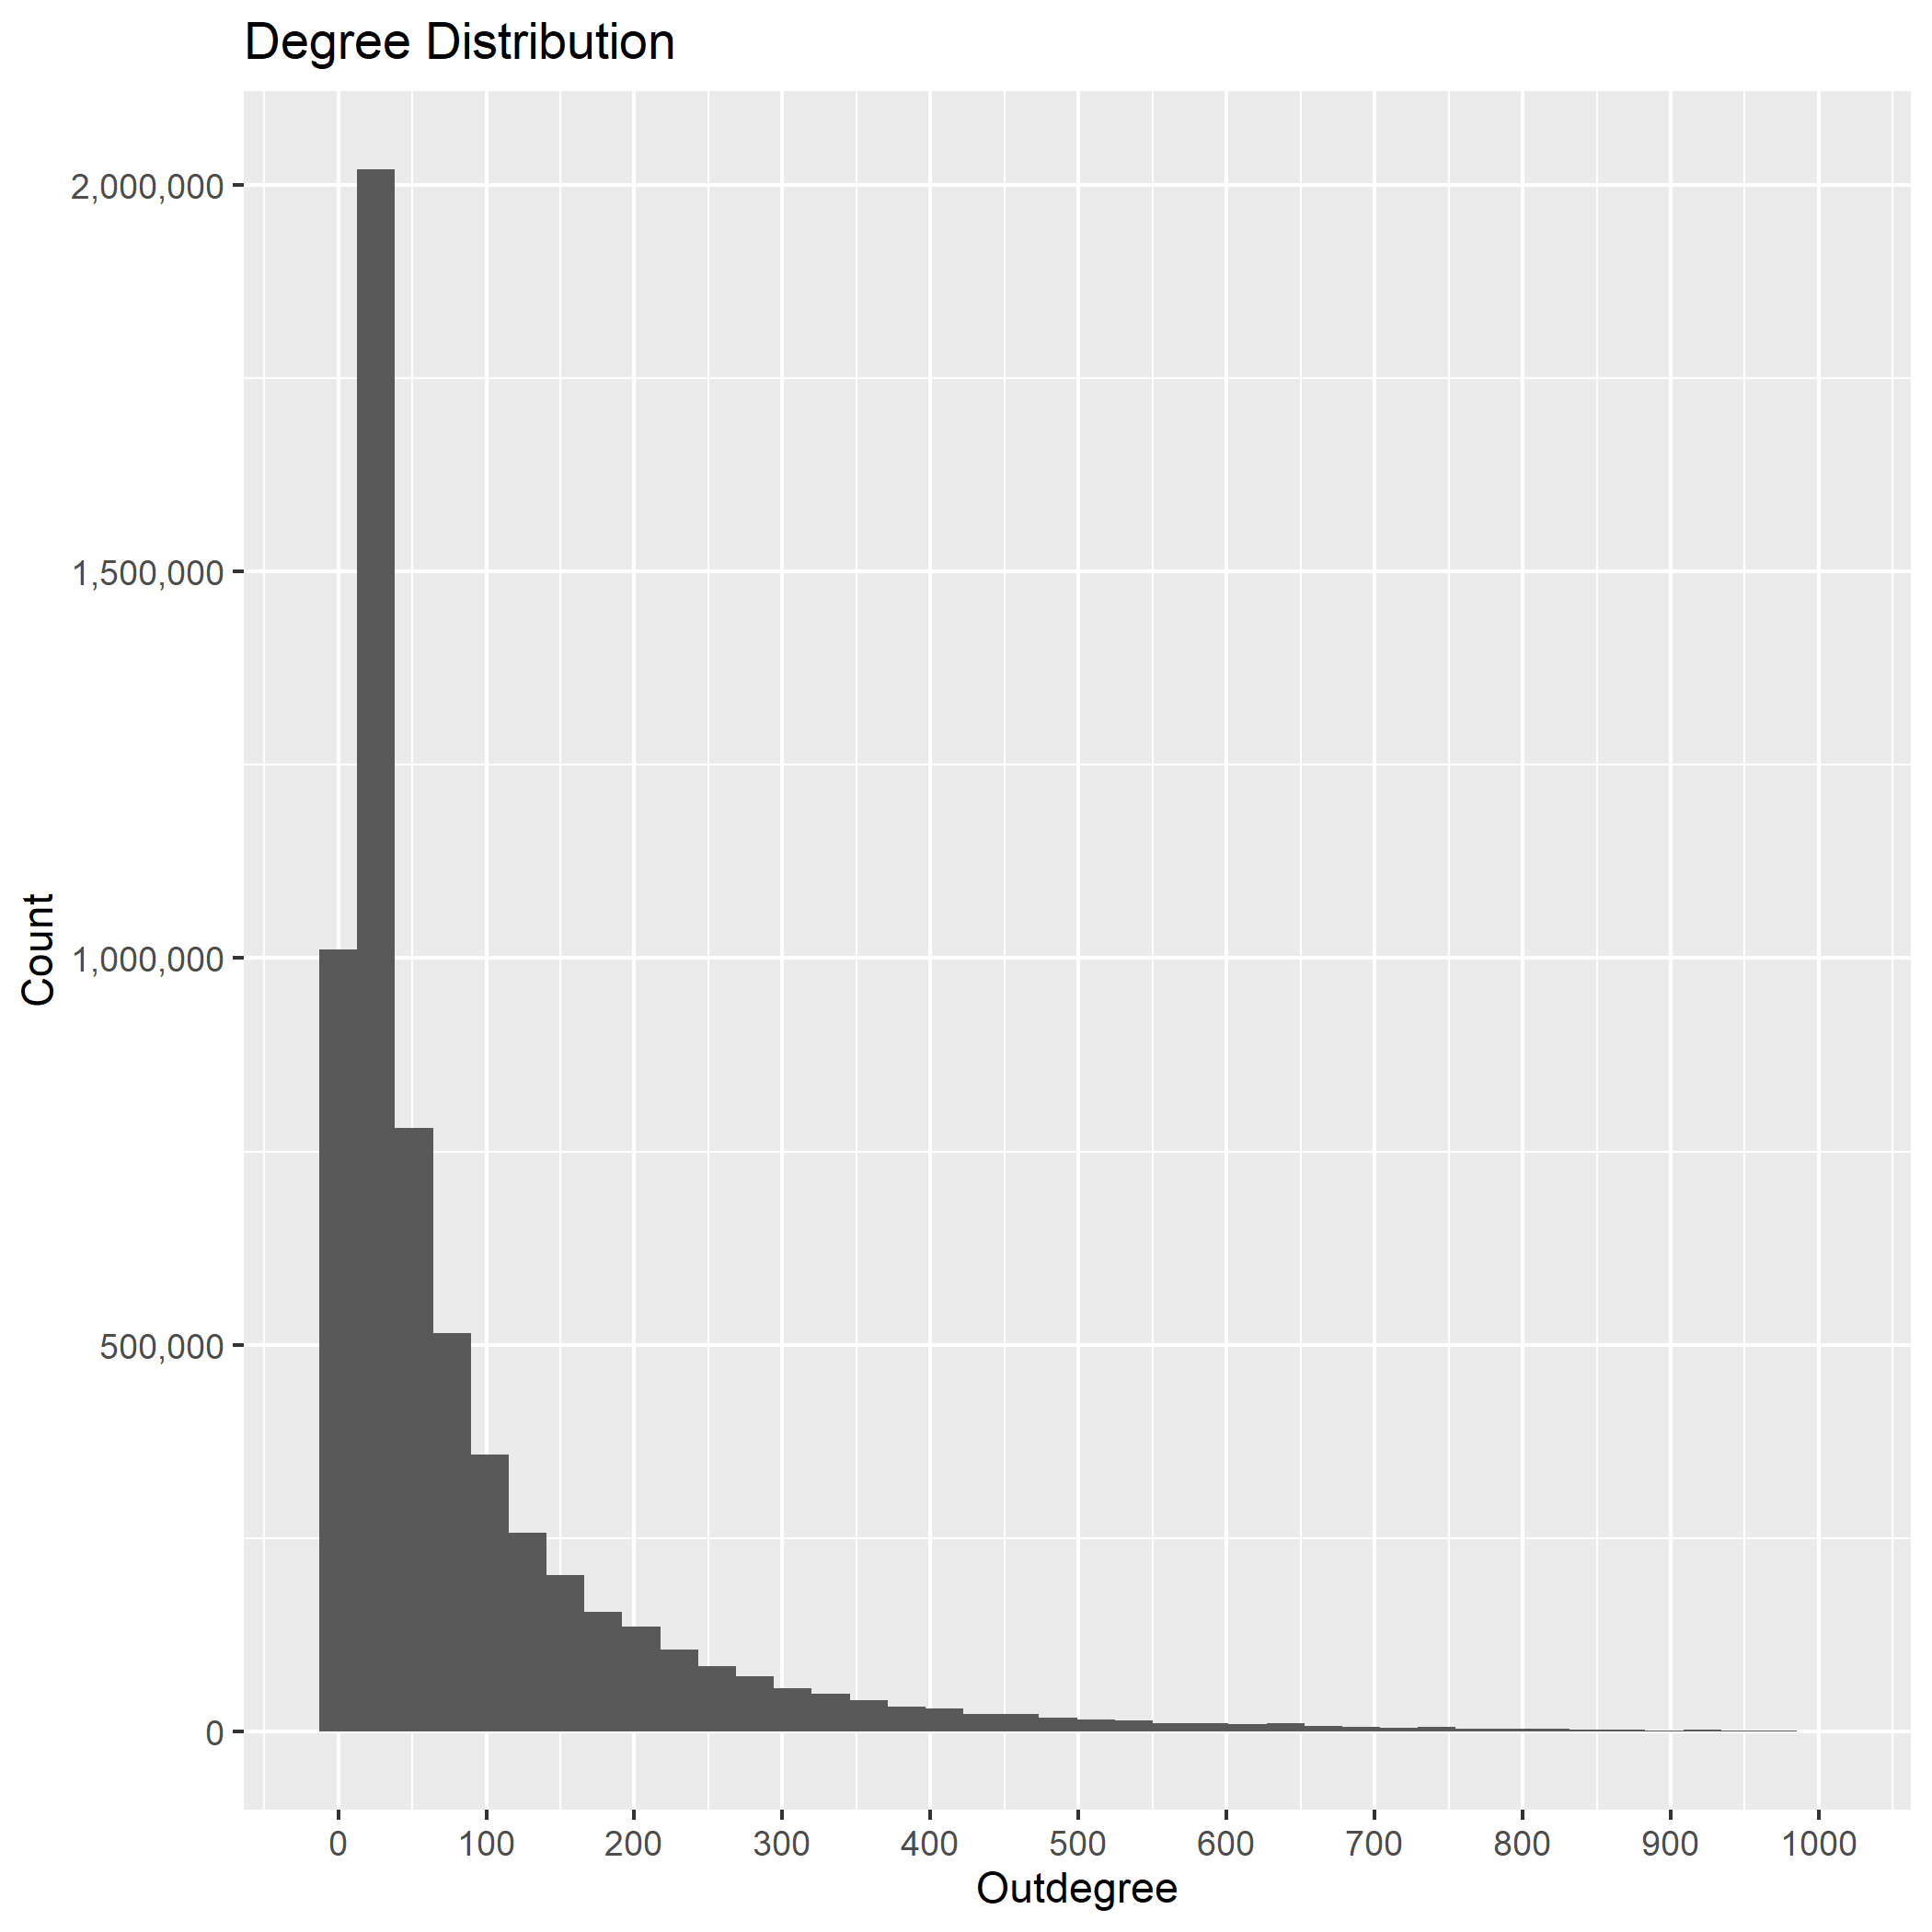
\includegraphics[width=6cm]{out_degree_dist}
    \caption{Outdegree Distribution}
    \label{fig:2figsB}
    \end{minipage}
\end{figure}


\section{Centrality}

A problem in graph theory is how to rank vertices in a graph by their importance. That is, figuring out which nodes in a network are central.
We evaluate three different metrics of centrality in the Wikipedia hyperlink graph.


\subsection{Degree Centrality}

Degree centrality is one of the simplest forms of centrality.
The indegree of a vertex in a directed graph is the number of edges that point to the vertex.
The outdegree of a vertex is the number of edges originating from that vertex.
To compute the indegree and outdegree we simply sum the rows and columns of the adjacency matrix.
% The adjacency matrix is not even required to compute degree centrality, 






\begin{figure}[H]
    \centering
    \caption{Highest Indegree}
    \begin{tabular}{llr}
        \toprule
        Article ID & Title & In Degree\\
        \midrule
        14919 & International\_Standard\_Book\_Number & 1305902\\
        48361 & Geographic\_coordinate\_system & 1151082\\
        25175562 & Virtual\_International\_Authority\_File & 904960\\
        18852926 & International\_Standard\_Name\_Identifier & 525539\\
        422994 & Digital\_object\_identifier & 471024\\
        \addlinespace
        3434750 & United\_States & 440874\\
        35412202 & Wikidata & 438109\\
        30463 & Taxonomy\_(biology) & 432978\\
        23538754 & Wayback\_Machine & 411661\\
        30890 & Time\_zone & 406023\\
        \addlinespace
        2987862 & Global\_Biodiversity\_Information\_Facility & 388044\\
        2855554 & IMDb & 339971\\
        39736 & Binomial\_nomenclature & 334349\\
        11039790 & Animal & 332711\\
        8439 & Diacritic & 322697\\
        \bottomrule
    \end{tabular}
\end{figure}
    
There are several pages in the Wikipedia network with excessive indegree compared to their outdegree. 
The article \textbf{International\_Standard\_Book\_Number} has an indegree of 1,322,167, but only an outdegree of 559. In fact, 20\% of all vertices in the graph have an edge connecting towards \textbf{International\_Standard\_Book\_Number}.
% This is because any article with a book in the references will contain a link to that article.
This is because of the automatic linking from references.
Any article with a citation that has an ISBN identifier will link to the page \textbf{International\_Standard\_Book\_Number}.
For similar reasons, the articles \textbf{Wayback\_Machine} and \textbf{OCLC} all have all have excessive indegree compared to their outdegree.



\subsection{Closeness Centrality}


The motivation for closeness centrality is to find how close one node is to different nodes in the network.
% The idea of closeness centrality is how close any node is to another node in the graph.


We are given a directed graph $G(V,E)$ with $n$ nodes and $m$ edges.
A directed graph is strongly connected if there is path between any two vertices. We assume that $G$ is strongly connected.
The distance $d(u, v)$ between vertices $u$ and $v$ is the shortest possible path between the vertices. Since $G$ is strongly connected, $d(u, v)$ always exists.


% Given a graph $G(V, E)$, the distance $d(u, v)$ between  vertices 
Eppstein defines closeness centrality $c_v$ of a vertex $v$ as,
\begin{equation*}
    c_v = \frac{n-1}{\sum_{u \in V}d(u,v)}
\end{equation*} 
The numerator $n-1$ normalizes the measure, making it comparable across different graphs.


The single source shortest path problem involves finding the distance from a single source to all other nodes in the graph. For undirected graphs, 
The all pairs shortest path problem is to find the shortest path between all possible pairs of vertices in the graph.
To find the exact closeness centrality for all nodes in the network, we must solve the all pairs shortest path problem. However, for large networks this is extremely computationally intensive. 
Eppstein provides a near-linear time approximation for centrality when the diameter is $O(\log n)$. That is, when the graph is a small world network. Since the Wikipedia hyperlink graph is a small world network, this algorithm is a good fit.

Then Eppstein presents the following algorithm RAND for computing closeness centrality,
\begin{enumerate}[1.]
    \item 
    Let k be the number of iterations needed to obtain the desired error bound.

    \item
    In iteration $i$, pick vertex $v_i$ uniformly at random from $G$ and solve the single source shortest path problem with $v_i$ as the source.

    \item 
    Let
    \begin{equation*}
        \hat{c}_ua = \frac{1}{\sum^k_{i=1} \frac{n d(v_i, u)}{k(n-1)}}
    \end{equation*}
    be the centrality estimator for vertex $u$.
\end{enumerate}

Since the graph is unweighted, we use a breadth first search to solve the SSSP problem.

\subsubsection{Results}

% A limitation of the implementation of the algorithm is that each breadth-first search takes 5 minutes to complete. Thus, to complete the process in a reasonable amount of time requires limiting the amount of iterations decreasing accuracy. This could be improved in future research by re-implementing the breadth first search in C, or another compiled language.

% The biggest difference with the closeness centrality metric is that the World War II metric is at the top.
% This is the only article that is not a country or a reference vertex to make the top of the list for the metrics.
% It's not surprising that World War II would be a central topic on Wikipedia, nearly all countries 



\begin{figure}[H]
    \caption[fig]{Closeness Centrality}
    \centering
    \begin{tabular}{rlr}
        \toprule
        Article ID & Title & Centrality \\
        \midrule
        14919 & International\_Standard\_Book\_Number & 0.5357142\\
        32927 & World\_War\_II & 0.5357142\\
        3434750 & United\_States & 0.5172413\\
        5843419 & France & 0.5172413\\
        23538754 & Wayback\_Machine & 0.5172413\\
        \addlinespace
        11867 & Germany & 0.4999999\\
        14532 & Italy & 0.4999999\\
        25391 & Russia & 0.4999999\\
        48361 & Geographic\_coordinate\_system & 0.4999999\\
        422994 & Digital\_object\_identifier & 0.4999999\\
        \addlinespace
        1057428 & Typographical\_error & 0.4999999\\
        26748 & Switzerland & 0.4838709\\
        31717 & United\_Kingdom & 0.4838709\\
        883885 & OCLC & 0.4838709\\
        5042916 & Canada & 0.4838709\\
    \bottomrule
\end{tabular}
\end{figure}

The World War II article is the only topic so far that is not a reference vertex or a country that has a high centrality. The importance of World War II within Wikipedia is not surprising. An unofficial Wikipedia game developed around 2010 called Clicks to Hitler, in which the participants try to reach the aforementioned page as quickly as possible.
Most articles link to at least one country, and most countries link to the World War II article.


\subsection{Katz Centrality}

The Katz Centrality measure was introduced in 1953 by Leo Katz. 
In this measure of centrality, the weighted count of incoming paths to each node determines it's importance in the network. The attenuation factor $\alpha$ changes how quickly the weights decrease the importance of walks.

We define Katz Centrality as,
\begin{equation*}
    C_{\textrm{Katz}}(i) = \sum_{j} (I_{ij} + \alpha A_{ij} + \alpha^2 A_{ij}^2 + \alpha^3 A_{ij}^3 + \dots).
\end{equation*}

Then,
\begin{align*}
    C_{\textrm{Katz}} &= (I + \alpha A + \alpha^2 A^2 + \alpha^3 A^3 + \dots) \begin{pmatrix}
        1 & \dots & 1
    \end{pmatrix}^T \\
    &= \sum^\infty_{n=1} (\alpha^n A^n)\begin{pmatrix}
    1 & 1 & \dots & 1
\end{pmatrix}^T \\ 
&= (I - \alpha A)^{-1} \begin{pmatrix}
    1 & 1 & \dots & 1
\end{pmatrix}^T 
\end{align*}
% https://www.youtube.com/watch?v=DfV-pjRTlLg

However, with extremely large matrices the inverse is difficult and imprecise to compute directly.
Therefore, we use power iteration to compute the measure instead.

\begin{figure}[H]
    \centering
    \begin{tabular}{llr}
        \toprule
        Article ID & Title & Katz Centrality\\
        \midrule
        14919 & International\_Standard\_Book\_Number & 0.0864162\\
        422994 & Digital\_object\_identifier & 0.0549040\\
        48361 & Geographic\_coordinate\_system & 0.0511208\\
        25175562 & Virtual\_International\_Authority\_File & 0.0387391\\
    23538754 & Wayback\_Machine & 0.0342068\\
    \addlinespace
    234930 & International\_Standard\_Serial\_Number & 0.0341706\\
    30890 & Time\_zone & 0.0285691\\
    5843419 & France & 0.0271659\\
    3434750 & United\_States & 0.0267877\\
    35412202 & Wikidata & 0.0253573\\
    \addlinespace
    48455863 & Semantic\_Scholar & 0.0251241\\
    503009 & PubMed & 0.0229752\\
    47548 & Daylight\_saving\_time & 0.0222805\\
    30463 & Taxonomy\_(biology) & 0.0222407\\
    19828134 & Plant & 0.0219509\\
    \bottomrule
    \end{tabular}
\end{figure}

We see that high degree nodes dominate in Katz Centrality.
The top five nodes that are listed all have very high indegree.
The majority of the highest scoring vertices seem to be reference nodes, such as \textbf{International\_Standard\_Serial\_Number}, \textbf{Virtual\_International Authority\_File}, and \textbf{PubMed}.
The only exceptions are the two country articles, \textbf{United\_States} and \textbf{France}.

\subsection{Conclusions}

The Katz Centrality and Indegree Centrality metrics


\section{Graph Radius \& Diameter}

The eccentricity of a vertex $v_i$ is the greatest distance between any other vertex $v$. That is, $e(v_i) = \max d(v_i, v)_{v \in V}$.

The radius of a graph is the minimum eccentricity of the entire graph, while the diameter of a graph is the maximum eccentricity.


Mathematically,
\begin{align*}
    r = \min e(v)_{v \in V} \\
    d = \max e(v)_{v \in V}
\end{align*}
where $r$ is the radius and $d$ is the diameter.

In the Wikipedia hyperlink graph the diameter can be conceptualized as given any article, how what is the maximum number of clicks to any other article in a shortest path. The radius can similarly be conceptualized as the minimum number of clicks to any other articles in a shortest path.


A naïve method of estimating the radius and the diameter is running multiple breadth first searches from random nodes and returning the minimum and maximum of the result. Boitmanis et. al presents a better approximation algorithm.

% https://sci-hub.se/https://dl.acm.org/doi/10.1007/11764298_9
Instead of starting the breadth first search from a uniformly random node, we start the breadth first search from the node furthest from the set of already processed nodes. This can be done in $O(n)$ time by keeping track of the results each breadth first search.

Using this search we can identify a tunnel of articles, from "Billboard Top Rock'n'Roll Hits: 1972" to "Billboard Top Hits: 1995". Where only a single path with 23 articles exists between the two articles.


\subsection{Results}

We estimate the radius and diameter of the 94.7\% of vertices that are strongly connected.
Using 20 iterations, the radius and diameter are both estimated at 33. That is, the eccentricity of the 20 tested nodes are all 33.
It is not clear if the estimated radius and diameter corresponds to the actual radius and diameter.

If the estimation is accurate, then from any article, the rest of the cluster is at most 33 clicks away.
This measure is robust to change against removing nodes. Removing the first 10,000 vertices with the highest indegree results in no change to the estimated radius and diameter. 


\section{Further Research}

One property of the hyperlink graph that isn't explored here is the order of the links. It is observable that repeatedly clicking the first link in nearly all articles will eventually lead to the Philosophy article. This is likely due to the definitional nature of the first paragraph in the article, that the first link in the article further abstracts the page.


% Another centrality measure that has not been implemented yet is betweeness centrality. This 


\section{Appendix}


\subsection{Katz Centrality}
\linespread{1}
\begin{lstlisting}[language=Python]
def katz_centrality(
graph,
alpha: float = 0.1,
beta: float = 1,
max_iter: int = 10000,
tol: float = 1.0e-6,
normalized: bool = True
):
    A = graph.adjacency.transpose()
    n = graph.size
    e = np.ones((n, 1))
    last = e.copy()
    for _ in range(max_iter):
        current = alpha * A.dot(last) + beta * e
        error = sum((abs(current[i] - last[i]) for i in range(n)))
        if error < n * tol:
            centrality = current.flatten().tolist()
            if normalized:
                norm = np.sign(sum(centrality)) * np.linalg.norm(centrality)
                return map(float, centrality / norm)
            else:
                return centrality
        last = current.copy()

    raise ConvergenceError(f"Failed to converge in {max_iter} iterations.")
\end{lstlisting}



\end{document}